\documentclass[conference]{IEEEtran}
\IEEEoverridecommandlockouts
% The preceding line is only needed to identify funding in the first footnote. If that is unneeded, please comment it out.
\usepackage{cite}
\usepackage{amsmath,amssymb,amsfonts}
\usepackage{algorithmic}
\usepackage{graphicx}
\usepackage{textcomp}
\usepackage{xcolor}
\usepackage{url}
\usepackage{hyperref}
\usepackage{float}
\usepackage{moresize}
\usepackage{booktabs}
\usepackage[para,online,flushleft]{threeparttable}


\makeatletter
\newcommand{\linebreakand}{%
  \end{@IEEEauthorhalign}
  \hfill\mbox{}\par
  \mbox{}\hfill\begin{@IEEEauthorhalign}
}
\makeatother



\def\BibTeX{{\rm B\kern-.05em{\sc i\kern-.025em b}\kern-.08em
    T\kern-.1667em\lower.7ex\hbox{E}\kern-.125emX}}
\begin{document}

\title{\textit{Cook County, IL:} Índices de precios de viviendas}

\author{%
\IEEEauthorblockN{Luis Alejandro Rubiano Guerrero}
\IEEEauthorblockA{202013482\\
\href{mailto:la.rubiano@uniandes.edu.co}{\texttt{la.rubiano@uniandes.edu.co}}}
\and
\IEEEauthorblockN{Andres Felipe Rosas Castillo}
\IEEEauthorblockA{202013471\\
\href{mailto:a.rosasc@uniandes.edu.co}{\texttt{a.rosasc@uniandes.edu.co}}}
\and
\IEEEauthorblockN{Carlos Andrés Castillo Cabrera}
\IEEEauthorblockA{202116837\\
\href{mailto:ca.castilloc1@uniandes.edu.co}{\texttt{ca.castilloc1@uniandes.edu.co}}}
}



\maketitle


\section{Introducción}

A través de este informe se construyen y se comparan \textbf{cuatro índices de precios de vivienda} para 
\textit{Cook County, Illinois} para el periodo comprendido entre 2000 y 2020. Las metodologías correspondientes a 
cada uno de los índices son las siguientes: (i) y (ii) índices de precios hedónicos, (iii) Índice de precios de la vivienda usada (IPVU), 
y (iv) estimador de efectos fijos con errores agrupados a nivel de propiedad. El objetivo de este informe es comparar y contrastar
 los resultados obtenidos a través de cada una de las metodologías, así como discutir las ventajas y desventajas de cada una de ellas.

En la sección II. se describe el conjunto de datos utilizado, así como el proceso de limpieza y tratamiento de los datos.
  La sección III. detalla la metodología utilizada para cada uno de los índices. En la sección IV. se presentan los resultados obtenidos, 
  así como un análisis comparativo entre los diferentes índices. Finalmente, en la sección V. se presentan las conclusiones del informe 
  y en la sección VI. se proporciona información adicional para la reproducibilidad del análisis.

\section{Datos y preparación}

\subsection{Descripción del conjunto de datos}

El conjunto de datos utilizado en este informe es \texttt{dataTaller01\_PriceIndeces.Rds}, 
el cual contiene información sobre ventas de viviendas en \textit{Cook County, Illinois} entre los años 2000 y 2020.
En total, el conjunto de datos contiene $427.649$ observaciones y $31$ variables. Estas variables incluyen 
el \texttt{pin} (identificador único de la propiedad), \texttt{year} (fecha de venta de la vivienda),
  \texttt{sale\_price} (precio de venta de la vivienda), \texttt{township\_code} (código local correspondiente al \textit{township} donde se ubica la propiedad),
  así como 27 covariables continuas y categóricas de características estructurales y de ubicación de las viviendas.

\subsection{Limpieza y tratamiento}

Se encontraron valores faltantes para $1060$ de las observaciones, en las variables 
\texttt{building\_sqft}, \texttt{num\_bedrooms}, \texttt{num\_rooms}, \texttt{num\_full\_baths},
\texttt{num\_half\_baths} y \texttt{num\_fireplaces}. Estas observaciones fueron eliminadas del conjunto de datos.

Adicionalmente, después de eliminar las anteriores observaciones, se encontraron $151.929$ observaciones con 
valores faltantes en la variable \texttt{land\_sqft}, lo cual representa aproximadamente el $36\%$ del total de las observaciones.
Estas fueron tratadas de manera diferente dependiendo de la metodología utilizada para construir los índices de precios de vivienda.

Adicionalmente se creó la variable \texttt{log\_sale\_price}, la cual corresponde al logaritmo natural del precio de venta de la vivienda, la 
cual es la variable dependiente de interés en los respectivos índices de precios.

\section{Metodología}

En todas las metodologías se normaliza el índice tomando como base el año 2000, es decir, el índice toma valor 100 en el año 2000.

\subsection{Índice hedónico}

Un índice hedónico se encuentra definido por la siguiente regresión.

\[ \log(P)_{it} = \sum_{t=t_0}^{T} \delta_t D_{it} + \sum_{j=1}^h \beta_j H_{ij} + \sum_{k=1}^n \beta_k N_{ik} + \mu_{it} \]

En donde:

\begin{itemize}
  \item $\log{P}_{it}$ es el logaritmo natural del precio de venta de la vivienda $i$ en el tiempo $t$, ($t = t_0, \ldots, T$).
  \item $D_{it}$ es una variable indicadora de la venta de la vivienda $i$ en el tiempo $t$.
  \item $H$ representa características estructurales de la vivienda.
  \item $N$ representa características de la ubicación de la vivienda.
  \item $\mu_{it}$ es el término de error, el cual se asume que es idénticamente distribuido, $\mu_{it} \sim N(0, \sigma^2)$.
\end{itemize}

En este caso estimamos dos índices hedónicos diferentes, en donde $t_0 = 2000$ y $T = 2020$. 

En el primer modelo las características estructurales $H$ son:

\texttt{class, year\_built, building\_sqft, land\_sqft, num\_bedrooms, num\_rooms, num\_full\_baths, num\_half\_baths, num\_fireplaces,
type\_of\_residence, construction\_quality, attic\_finish, garage\_attached, garage\_area\_included, garage\_size, garage\_ext\_wall\_material, attic\_type, basement\_type, ext\_wall\_material, central\_heating, basement\_finish, roof\_material, renovation, recent\_renovation, porch, central\_air}

y en el segundo modelo son las mismas características estructurales pero sin incluir \texttt{land\_sqft}.

en ambos modelos las características de ubicación $N$ son:

\texttt{township\_code, site\_desirability}. 

La diferencia entre los modelos es que en el primero se incluye la covariable 
\texttt{land\_sqft}, pero se eliminan las observaciones con valores faltantes en esta variable,
mientras que en el segundo modelo no se incluye esta covariable, pero se utilizan todas las observaciones.

Asimismo, de manera preventiva se agrupan los errores a nivel de \texttt{township\_code}, es decir, se asume que los errores pueden estar correlacionados 
dentro de cada \textit{township}, pero son independientes entre diferentes \textit{townships}.

Finalmente, para estimar los índices se calcula $I_t = 100 \cdot \exp(\beta_t - \beta_{2000}) = 100 \cdot \exp(\beta_t)$, y se calculan sus errores estándar utilizando el método del delta, 
es decir $\text{var}(I_t) \approx (100 \cdot \exp(\beta_t)) \cdot \text{var}(\beta_t)$.


\subsection{Índice de ventas repetidas (IPVU)}

En este índice requiere identificar viviendas que hayan sido vendidas por lo
menos dos veces dentro del periodo de estudio, basado en la metodología de \textit{Case y Shiller} (1989).

Por lo tanto, filtramos el conjunto de datos para incluir únicamente aquellas viviendas que han sido vendidas más de una vez
durante el periodo de estudio y que no hayan presentado modificaciones significativas en
su estructura física. Para lo último, descartamos las ventas tales que la variable \texttt{recent\_renovation} sea \texttt{TRUE}. 
La base de datos resultante tiene $233.233$ observaciones. 

En este modelo se asume que el comportamiento del precio de la misma vivienda
$P_t$ es un proceso estocástico dado por:

\[ \ln(P_{i,t}) = \beta_t + H_{i,t} + N_{i, t}\] 

En donde $\beta_t$ corresponde al índice del precio, $H_{i, t}$ es una caminata aleatoria
gaussiana que describe como el cambio del precio de una vivienda individual se desvía en
el tiempo respecto a la variación del índice de mercado, y $N_{i, t}$ son errores que se asumen 
normales y representa las diferencias idiosincrásicas de las propiedades en un momento
del tiempo.

Para este índice se crea una variable que representa el cambio porcentual total en el precio de una vivienda entre dos transacciones. Esta variable se define como:

\begin{align*}
  \Delta V_i &= \ln(P_{i,t})-\ln(P_{i,s})\\
  &= \beta_t - \beta_s + H_{i,t} - H_{i,s} + N_{i,t} - N_{i,s}\\
\end{align*}

Sobre los términos de perturbación se asume que 

\begin{align*}
  \mathbb{E}[H_{i,t} - H_{i, s}] &= 0 (\text{media cero}) \\
  \text{Var}(H_{i,t} - H_{i, s}) &= A(t-s) + B(t-s)^2 (\tiny\text{var cuadrática en el tiempo})\\
  \mathbb{E}[N_{i, t}] &= 0 (\text{media cero})\\
  \text{Var}(N_{i, t}) &= c (\text{varianza constante})\\
  \mathbb{E}[H_{i,t}N_{i, t}] &= 0 (\text{independencia})
\end{align*}

Partiendo de lo anterior, los índices de precios se estiman en tres etapas:

\begin{enumerate}
  \item Primera etapa: Se estiman los $\beta$ iniciales y los errores.
  
  Para una venta repetida de una vivienda $i$ se estima el cambio porcentual de la siguiente forma:

  \begin{align*}
    \Delta V_i &= \sum_{t=t_0}^{T} \ln(P_{i,t}) D_{it}\\
    &= \sum_{t=t_0}^{T} \beta_t D_{it} + \varepsilon_{i}
  \end{align*}

  En donde $D_{it}$ es una variable indicadora que toma valor 
  $1$ cuando el precio de la vivienda $i$ es
  observado por segunda vez en $t$, $-1$ si el precio de la vivienda $i$ fue observado por primera
  vez en $t$, y cero de lo contrario. 

  Aquí $\beta_t$ se estima a través de mínimos cuadrados ordinarios.

  \item Segunda etapa: Se estima la varianza de la caminata aleatoria.
  
  En esta etapa se estiman los coeficientes $A$, $B$ y $c$ a través de mínimos cuadrados ordinarios,
  mediante la expresión:

  \[ \mathbb{E}[\varepsilon_i^2] = A(t-s) + B(t-s)^2 + c \]

  Es decir, se estima la varianza de los errores al cuadrado como función cuadrática del tiempo entre ventas.
  En este caso $\mathbb{E}[\varepsilon_i^2]$ es la varianza muestral de los errores estimados en la primera etapa.
  Si los coeficientes estimados $A$ y $B$ son positivos y significativos, se debe continuar con la tercera etapa, 
  en tal caso la raíz cuadrada de los valores estimados por la ecuación se utiliza para ponderar por mínimos cuadrados generalizados.

  \item Tercera etapa: Se re-estiman los $\beta$ utilizando mínimos cuadrados generalizados.
  
  Es decir, se estima 

  \[ \cfrac{\Delta V_i}{\sqrt{\hat{\varepsilon_i^2}}} = \sum_{t=t_0}^{T} \cfrac{\beta_t}{\sqrt{\hat{\varepsilon_i^2}}} D_{it} + \cfrac{\varepsilon_{i}}{\sqrt{\hat{\varepsilon_i^2}}} \]

  Posteriormente, los indices y los errores estándar se calculan de forma similar a la metodología de índices hedónicos.

\end{enumerate}


\subsection{Estimador de efectos fijos con errores agrupados}

El estimador de efectos fijos (FE) explota la variación \emph{intra-propiedad} para aislar cambios en el precio no explicados por características inobservables \emph{invariantes en el tiempo} de cada vivienda. 
Para esto se filtraron las propiedades con al menos dos ventas en el periodo de estudio, resultando en $233.388$ observaciones.

La especificación es:

\[ \log(P)_{it} = \sum_{t=t_0}^{T} \delta_t D_{it} + \sum_{j=1}^h \beta_j Z_{ij} + \alpha_i + \epsilon_{it} \]

En donde:

\begin{itemize}
  \item $D_{it}$ es una variable indicadora de la venta de la vivienda $i$ en el tiempo $t$.
  \item $Z$ representa características estructurales y de ubicación de la vivienda que varían en el tiempo, en particular 
  \texttt{building\_sqft, num\_bedrooms, num\_rooms, num\_full\_baths, num\_half\_baths, renovation, recent\_renovation, central\_air, central\_heating, garage\_attached, garage\_size, attic\_finish, basement\_finish}.
  \item $\alpha_i$ es el efecto fijo de la vivienda $i$.
  \item $\epsilon_{it}$ es el término de error, el cual se asume que es idénticamente distribuido, $\epsilon_{it} \sim N(0, \sigma^2)$.
\end{itemize}

En este caso asumimos que los errores pueden estar correlacionados dentro de cada propiedad a lo largo del tiempo, pero son independientes entre diferentes propiedades, y por lo tanto 
agrupamos los errores a nivel de propiedad.

Aquí los índices y los errores estándar se calculan de forma similar a la metodología de índices hedónicos.

\section{Resultados y análisis}

\subsection{Gráfica comparativa de índices}

\begin{figure}[H]
  \centering
  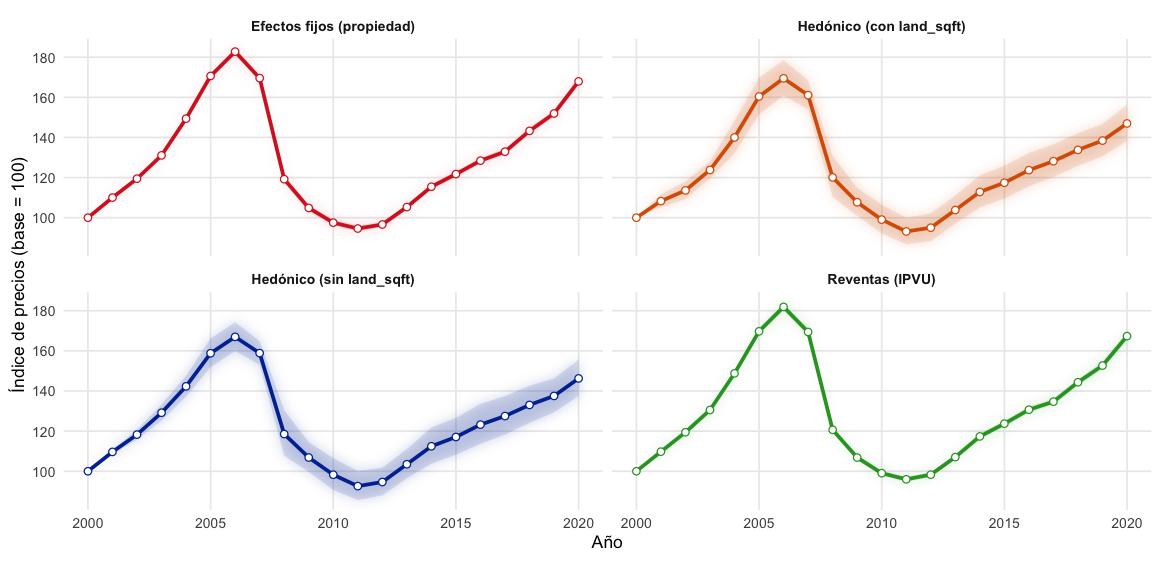
\includegraphics[width=0.48\textwidth]{../figures/grafica1.png}
  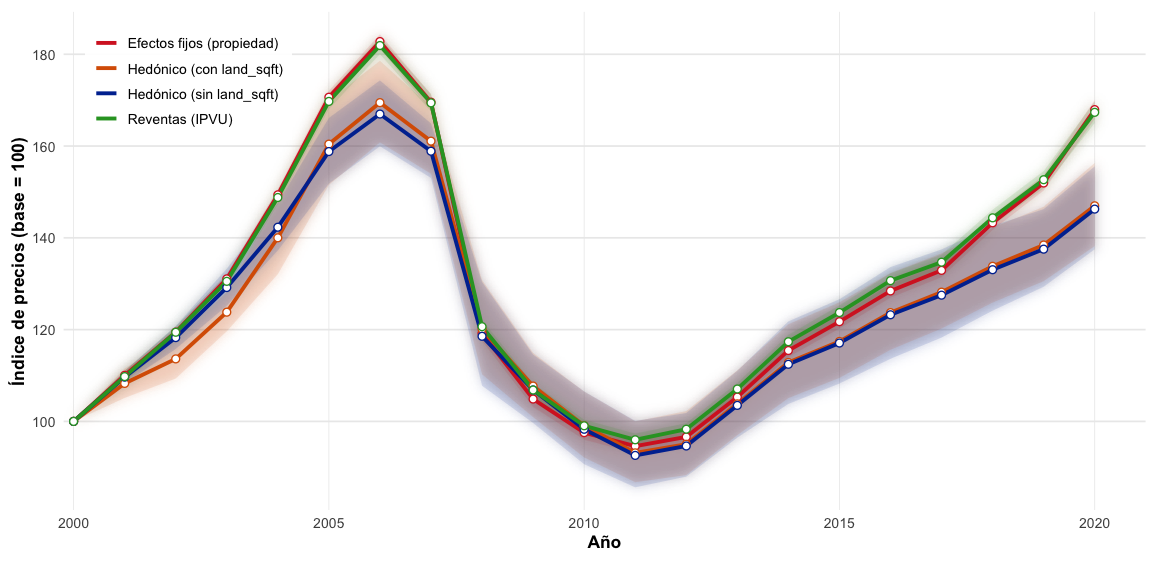
\includegraphics[width=0.48\textwidth]{../figures/grafica2.png}
  \caption{Comparación de los cuatro índices de precios de vivienda.}
  \label{fig:indices_comparacion}
\end{figure}

\subsection{Comparación cuantitativa}

\begin{table}[H]
\tiny
\centering
\caption{Comparación de índices y modelos (2000–2020)}
\begin{threeparttable}
\begin{tabular}{lcccc}
\toprule
Año & Efectos fijos (propiedad) & Hedónico (sin land\_sqft) & Hedónico (con land\_sqft) & Reventas (IPVU) \\
\midrule
2000 & 0.0000 (0.0000) & 0.0000 (0.0000) & 0.0000 (0.0000) & 0.0000 (0.0000) \\
2001 & 0.0956 (0.0047) & 0.0921 (0.0063) & 0.0793 (0.0151) & 0.0931 (0.0059) \\
2002 & -0.1777 (0.0051) & 0.1678 (0.0108) & 0.1277 (0.0196) & 0.1775 (0.0057) \\
2003 & 0.2705 (0.0043) & 0.2560 (0.0159) & 0.2136 (0.0175) & 0.2664 (0.0054) \\
2004 & 0.4013 (0.0042) & 0.3528 (0.0186) & 0.3368 (0.0298) & 0.3979 (0.0053) \\
2005 & 0.5344 (0.0042) & 0.4625 (0.0230) & 0.4726 (0.0291) & 0.5290 (0.0049) \\
2006 & 0.6031 (0.0044) & 0.5127 (0.0219) & 0.5274 (0.0268) & 0.5983 (0.0053) \\
2007 & 0.5282 (0.0052) & 0.4629 (0.0487) & 0.4767 (0.0230) & 0.5271 (0.0058) \\
2008 & 0.1756 (0.0071) & 0.1701 (0.0486) & 0.1831 (0.0346) & 0.1877 (0.0063) \\
2009 & 0.0476 (0.0085) & 0.0663 (0.0356) & 0.0715 (0.0369) & 0.0476 (0.0070) \\
2010 & -0.0249 (0.0081) & -0.0173 (0.0416) & -0.0710 (0.0362) & -0.0096 (0.0068) \\
2011 & -0.0548 (0.0083) & -0.0760 (0.0399) & -0.0511 (0.0374) & -0.0403 (0.0067) \\
2012 & -0.0343 (0.0075) & -0.0551 (0.0374) & 0.0376 (0.0346) & -0.0172 (0.0069) \\
2013 & 0.0517 (0.0064) & 0.0343 (0.0359) & 0.0201 (0.0318) & 0.0681 (0.0064) \\
2014 & 0.1436 (0.0064) & 0.1174 (0.0408) & 0.1260 (0.0370) & 0.1442 (0.0057) \\
2015 & 0.1970 (0.0063) & 0.1577 (0.0400) & 0.1651 (0.0375) & 0.2127 (0.0065) \\
2016 & 0.2502 (0.0058) & 0.2089 (0.0413) & 0.2127 (0.0345) & 0.2675 (0.0067) \\
2017 & 0.2845 (0.0057) & 0.2430 (0.0354) & 0.2481 (0.0326) & 0.2978 (0.0064) \\
2018 & 0.3595 (0.0057) & 0.2856 (0.0354) & 0.2792 (0.0318) & 0.3196 (0.0062) \\
2019 & 0.4184 (0.0055) & 0.3187 (0.0354) & 0.3215 (0.0296) & 0.4230 (0.0066) \\
2020 & 0.5185 (0.0064) & 0.3802 (0.0351) & 0.3851 (0.0315) & 0.5149 (0.0072) \\
\bottomrule
\end{tabular}
\begin{tablenotes}
\footnotesize
\item Nota: Se reportan los coeficientes anuales (en log-precios relativos) y, entre paréntesis, los errores estándar según cada método. 
\item Los modelos corresponden al estimador de efectos fijos, dos versiones del modelo hedónico, y el índice de precios de reventas (IPVU).
\end{tablenotes}
\end{threeparttable}
\end{table}

\begin{table}[H]
\tiny
\centering
\caption{Índices de precios por modelo (2000–2020)}
\begin{threeparttable}
\begin{tabular}{lcccc}
\toprule
Año & Efectos fijos (propiedad) & Hedónico (sin land\_sqft) & Hedónico (con land\_sqft) & Reventas (IPVU) \\
\midrule
2000 & 100.00 & 100.00 & 100.00 & 100.00 \\
2001 & 110.03 & 109.64 & 108.28 & 109.76 \\
2002 & 119.45 & 118.26 & 113.62 & 119.42 \\
2003 & 131.06 & 129.17 & 123.80 & 130.52 \\
2004 & 143.05 & 142.35 & 140.42 & 148.79 \\
2005 & 170.64 & 158.80 & 160.42 & 169.72 \\
2006 & 182.77 & 166.97 & 169.46 & 181.91 \\
2007 & 169.56 & 158.87 & 161.07 & 169.41 \\
2008 & 119.19 & 118.55 & 120.09 & 120.64 \\
2009 & 97.55  & 106.86 & 107.70 & 109.04 \\
2010 & 97.55  & 98.29  & 99.06  & 99.04 \\
2011 & 94.60  & 92.59  & 93.14  & 95.99 \\
2012 & 96.62  & 94.64  & 95.02  & 98.30 \\
2013 & 110.45 & 107.42 & 108.32 & 107.06 \\
2014 & 115.45 & 112.45 & 115.06 & 117.35 \\
2015 & 121.73 & 117.08 & 117.42 & 123.71 \\
2016 & 128.42 & 123.23 & 123.70 & 130.67 \\
2017 & 132.91 & 127.51 & 128.16 & 134.68 \\
2018 & 139.43 & 133.06 & 133.79 & 144.35 \\
2019 & 151.49 & 137.53 & 138.43 & 152.66 \\
2020 & 167.93 & 146.26 & 146.98 & 167.35 \\
\bottomrule
\end{tabular}
\begin{tablenotes}
\footnotesize
\item Nota: Los valores corresponden a índices de precios relativos (base 2000 = 100) estimados mediante diferentes especificaciones: efectos fijos a nivel de propiedad, modelos hedónicos con y sin la variable \texttt{land\_sqft}, y el índice de reventas (IPVU).
\end{tablenotes}
\end{threeparttable}
\end{table}


\begin{table}[H]
\centering
\caption{IPVU — Etapa 2: Modelo cuadrático para la varianza en función del \textit{gap}}
\begin{threeparttable}
\begin{tabular}{lccc}
\toprule
& \multicolumn{3}{c}{\textbf{VD: }$\widehat{\varepsilon_i^2}$} \\
\cmidrule(lr){2-4}
 & Coeficiente & Error estándar & t \\
\midrule
Intercepto      & 0.3913$^{***}$ & (0.004281) &  91.41 \\
gap             & $-0.03649^{***}$ & (0.001355) & $-26.94$ \\
$gap^{2}$       & 0.001544$^{***}$ & (0.0000811) &  19.04 \\
\midrule
Observaciones   & \multicolumn{3}{c}{133{,}559} \\
RSE (residual)  & \multicolumn{3}{c}{0.628 \quad (gl = 133{,}556)} \\
$R^{2}$         & \multicolumn{3}{c}{0.009864} \\
$R^{2}$ ajustado& \multicolumn{3}{c}{0.009849} \\
Estadístico F   & \multicolumn{3}{c}{665.3 \; (df = 2; 133{,}556), \; $p<2.2\times10^{-16}$} \\
\bottomrule
\end{tabular}
\begin{tablenotes}
\footnotesize
\item Notas: Errores estándar entre paréntesis. $^{***}p<0.001$, $^{**}p<0.01$, $^{*}p<0.05$.
\item Especificación: $\mathbb{E}[\varepsilon_i^2\mid gap_i]=\alpha+\beta\,gap_i+\gamma\,gap_i^2$ (MCO).
\end{tablenotes}
\end{threeparttable}
\end{table}

\begin{table}[H]
\centering
\caption{Comparación del $R^2$ entre modelos de precios}
\begin{threeparttable}
\begin{tabular}{lcc}
\toprule
\textbf{Modelo} & \textbf{$R^2$} \\
\midrule
Reventas (IPVU) & 0.2531883 \\
Hedónico (con \textit{land\_sqft}) & 0.616803 \\
Hedónico (sin \textit{land\_sqft}) & 0.623158 \\
Efectos fijos (propiedad) & 0.867540 \\
\bottomrule
\end{tabular}
\begin{tablenotes}
\footnotesize
\item \textit{Nota:} El estadístico $R^2$ refleja el poder explicativo de cada modelo sobre la variación en el logaritmo del precio de venta. 
\end{tablenotes}
\end{threeparttable}
\end{table}



\subsection{Discusión}

Las cuatro metodologías cuentan esencialmente la misma historia del mercado de Cook County: auge a mediados de los 2000, corrección en 2008-2011 y recuperación sostenida desde 2013 hasta 2020. En la figura conjunta, las bandas de confianza se intersecan durante casi todo el periodo y los puntos de giro coinciden, lo que sugiere que la señal del ciclo es robusta al método.

\paragraph{Hedónicos: con y sin \texttt{land\_sqft}.}
Los dos hedónicos trazan prácticamente la misma trayectoria anual. El modelo \emph{sin} \texttt{land\_sqft} aprovecha 426{,}589 ventas (frente a 274{,}660 \emph{con} \texttt{land\_sqft}) y, aun así, replica el perfil temporal. En ajuste in–sample muestra una ligera ventaja (Adj.\(R^2 \approx 0.623\)) respecto al que incluye \texttt{land\_sqft} (Adj.\(R^2 \approx 0.617\)), mejora atribuible sobre todo a un mayor número de muestras. Los coeficientes nuance son económicamente razonables: más área construida y más baños elevan el precio. Cuartos/dormitorios pierden relevancia al controlar por metraje. El efecto de \texttt{land\_sqft} es positivo pero pequeño (1{,}000 ft\(^2\) adicionales \(\sim\) 0.5\% más precio), consistente con que localización y área edificada explican más del valor.

\paragraph{Reventas (IPVU) y efectos fijos por propiedad.}
El IPVU reproduce la misma dinámica con oscilaciones algo más marcadas (propio de comparar la \emph{misma} vivienda en dos fechas) y, al excluir reventas con remodelación reciente, actúa como ancla del ciclo. El modelo con efectos fijos por propiedad entrega una serie anual alineada con las anteriores: su \(R^2\) total elevado (\(\approx 0.868\)) refleja la heterogeneidad fija absorbida por el identificador del predio, mientras que el de IPVU \(R^2 \approx 0.30\) indica que los cambios intra–vivienda explican una fracción relevante, pero el pulso del ciclo lo capturan sobre todo las dummies de año.

\paragraph{Comparación de desempeño.}
En dinámica temporal, ninguna especificación “domina”: las trayectorias prácticamente se superponen. En precisión y cobertura, el hedónico \emph{sin} \texttt{land\_sqft} resulta el balance más atractivo: mayor muestra (426{,}589 vs.\ 274{,}660) y mejor ajuste in–sample (Adj.\(R^2\approx 0.623\)) frente a \(0.617\), con bandas de confianza ligeramente más estrechas y sin cambiar la forma del ciclo. IPVU y efectos fijos, al basarse en reventas, operan sobre subconjuntos menores y pueden mostrar intervalos algo más amplios en algunos años; aun así, su trayectoria central coincide con la de los hedónicos.

\paragraph{Ventajas y desventajas.}
El hedónico con \texttt{land\_sqft} identifica explícitamente la contribución del lote, pero reduce la muestra en torno a 40\% y no mejora la trayectoria ni el ajuste. El hedónico sin \texttt{land\_sqft} gana cobertura y precisión con un índice prácticamente idéntico, a costa de no separar suelo y edificación. El IPVU controla calidad fija y valida los puntos de giro, aunque depende de inmuebles que se revenden y puede estar expuesto a remodelaciones no observadas. Los efectos fijos por propiedad absorben toda la heterogeneidad invariante del predio y confirman la dinámica en el subconjunto repetido, pero no son directamente comparables con MCO sobre la muestra completa.



\section{Conclusiones}

El análisis comparativo de las cuatro metodologías aplicadas, dos modelos hedónicos, el índice de precios de viviendas usadas (IPVU) y el estimador de efectos fijos por propiedad, muestra una notable coherencia en la identificación de los ciclos del mercado inmobiliario de \textit{Cook County, Illinois} entre 2000 y 2020. Todas las series reflejan un comportamiento común: crecimiento sostenido en la primera mitad de los años 2000, contracción pronunciada entre 2008 y 2011 asociada a la crisis financiera, y una recuperación gradual y persistente a partir de 2013.

Metodológicamente, el modelo de efectos fijos alcanza el mayor poder explicativo ($R^2 = 0.87$), al capturar heterogeneidad inobservable a nivel de vivienda. Sin embargo, esta precisión se logra sobre una submuestra de propiedades con múltiples transacciones. El índice de reventas (IPVU), aunque basado en un enfoque similar, presenta un menor ajuste ($R^2 = 0.25$) debido a su naturaleza más restrictiva, pero conserva la ventaja de reflejar cambios de precios \emph{reales} sobre las mismas unidades, sirviendo como una referencia sólida para validar los patrones temporales.

Por su parte, los modelos hedónicos, con y sin la variable \texttt{land\_sqft}, logran resultados prácticamente indistinguibles en términos de tendencia, destacando que la exclusión de dicha variable amplía sustancialmente la cobertura muestral sin deteriorar el ajuste ni alterar la trayectoria del índice. Esto sugiere que las variables estructurales y de localización capturan de forma suficiente las variaciones relevantes del precio, y que el área del terreno tiene un papel marginal en la dinámica temporal agregada.

\section{Información adicional de reproducibilidad}

Haciendo click en \href{https://github.com/larubiano0/HW1-Urban-Economics-part1}{\textit{este enlace}} se puede acceder al repositorio de GitHub que contiene el código utilizado para realizar el análisis y generar los resultados presentados en este informe.


\end{document}
